\documentclass{article}
\usepackage[utf8]{inputenc}
% \usepackage[english,greek]{babel}
\usepackage[unicode]{hyperref}
\usepackage[LGR, T1]{fontenc}
\usepackage{amsfonts, alphabeta, amssymb}
\usepackage[none]{hyphenat}
\usepackage[bottom]{footmisc}
\usepackage{amsmath, slashed, graphicx, physics, tikz, braket, caption, subfig, comment, geometry, multicol, lipsum, fancyhdr, tcolorbox, siunitx, authblk, xcolor, abstract, float, indentfirst, xfrac, cancel, bbold, appendix, tikz, tikz-feynman, tensor, multirow, makecell, algpseudocode, algorithmicx, algorithm, changepage, adjustbox, lscape}
\usepackage[style=numeric-comp,sorting=none]{biblatex}
\addbibresource{references.bib}
\setcounter{secnumdepth}{3}
\setcounter{tocdepth}{3}
\title{\textbf{
        Study of a new kinematic weighting algorithm for the measurement of CP asymmetries in charm decays}
        \\
        LHCb Collaboration
}
\author{
        Georgios Christou\thanks{Source code available at: \url{https://github.com/GiorgosChr/CERN_Summer_Student_Programme_2023}}
        \\
        Supervisors: Dr.\@ Federico Betti and Prof.\@ Angelo Carbone
}
\date{
        August 2023
}

\begin{document}
        \begin{figure}[t]
                \centering
                \hypersetup{hidelinks} % Remove hyperlink border only for this figure
                \subfloat{\href{https://home.cern/}{
\includegraphics[height=3.5cm]{../.images/CERN_logo.png}}}
                \hspace{1cm}
                \subfloat{\href{https://lhcb.web.cern.ch/}{
\includegraphics[height=3.5cm]{../.images/Lhcb-logo-new.svg.png}}}
        \end{figure}

        \maketitle
        \thispagestyle{empty}

        \begin{abstract}
                We investigate the asymmetries that occur in charm decays at the LHCb, specifically we study $D^{\star+}\to D^0\pi^+$ and $D^{\star-}\to \bar{D}^0\pi^-$ where $D^0\to K^-K^+$ or $D^0\to \pi^-\pi^+$.
                We study the effect of $CP$ and detection asymmetries on MC samples generated via RapidSim and implement a new kinematic weighting function which allows us to keep events that are otherwise discarded from LHCb data, since they are associated with large detection asymmetries.
        \end{abstract}

        
        \pagebreak

        \pagenumbering{arabic}
        % \tableofcontents
        % \pagebreak

        \section{Introduction}
        We investigate charm decays and specifically the $D^\star$ meson.
        By studying the differences between $D^{\star +}$ and $D^{\star -}$ decays we can estimate the $CP$ asymmetry.
        Specifically, we are interested in
        \begin{eqnarray}
                &D^{\star+}\to D^0\pi^+ \text{ and } D^{\star-}\to \bar{D}^0\pi^-, \nonumber\\
                &D^0 \to K^-K^+ \text{ and } D^0 \to \pi^-\pi^+
        \end{eqnarray}
        decay modes where we refer to the $\pi^\pm$ as \textit{soft pion}.

        The total asymmetry one observes at an experiment is a combination of multiple asymmetries.
        Namely, the total asymmetry consists of a \textit{production}, a \textit{CP} and a \textit{detection} asymmetry, however, throughout this project we are not interested in production asymmetries.
        The $CP$ asymmetry is associated with the decay differences of matter and anti-matter, while the detection asymmetry is associated with the differences in detecting the positive and negative soft pions $(\pi_s^\pm)$.
        
        We can calculate the \textit{total asymmetry} by
        \begin{equation}
                A_\text{total} = \frac{A_{CP} + A_D}{1 + A_{CP}A_D},
        \end{equation}
        where $A_{CP}$ and $A_D$ are the $CP$ and \textit{integrated detection} asymmetries.
        The latter is calculated using
        \begin{equation}
                A_D = \frac{\int \dd \vec{p} N(\vec{p})A_D(\vec{p})}{\int \dd \vec{p} N(\vec{p})}
        \end{equation}
        where $N(\vec{p})$ and $A_D(\vec{p})$ are the momentum-dependent number of events and detection asymmetry respectively.
        We can however, approximate the total asymmetry up to $\mathcal{O}(10^{-6})$ if $A_{CP}$ is up to $\mathcal{O}(10^{-3})$ and $A_D$ up to $\mathcal{O}(10^{-2})$ as
        \begin{equation}
                A_\text{total} = A_{CP} + A_{D}
        \end{equation}

        The observable we can calculate from an experiment is the \textit{total asymmetry difference} between the two modes which approximately gives us
        \begin{eqnarray}
                \begin{split}
                        \Delta A_\text{total} & = A^{KK}_\text{total} - A^{\pi\pi}_\text{total}\\
                        & = \Delta A_{CP} - \Delta A_D,
                \end{split}
        \end{eqnarray}
        however, we are interested in $\Delta A_{CP}$, thus, we require a method to eliminate $\Delta A_D$.

        At the LHCb one observes large pion detection asymmetries that are associated with specific kinematic regions, which so far have been discarded, thus reducing the statistics.
        We can, however, introduce a \textit{weighting function} based on $D^0$ kinematics
        \begin{equation}
                \label{eq:weighting}
                Q(\vec{p}_{D^\star}, \vec{p}_{\pi_s}) \simeq \frac{\Gamma_{D^0}^{\pi\pi}(\vec{p}_{D^\star} - \vec{p}_{\pi_s}) + \Gamma_{\bar{D}^0}^{\pi\pi}(\vec{p}_{D^\star} - \vec{p}_{\pi_s})}{\Gamma_{D^0}^{KK}(\vec{p}_{D^\star} - \vec{p}_{\pi_s}) + \Gamma_{\bar{D}^0}^{KK}(\vec{p}_{D^\star} - \vec{p}_{\pi_s})}
        \end{equation}
        where $\Gamma_{D^{0}/\bar{D}^0}^{\pi\pi/KK}$ are the normalized distributions of $D^0$ candidates.
        Here, the $D^0$ candidates are reconstructed using the $D^\star$ and $\pi_s$, however, this weighting function does not allow for events associated with large detection asymmetries to be included to the analysis since it is biased.
        A new weighting function which is much more effective comes from reconstructing $D^0$ candidates without associating them with $\pi_s$, thus, the weighting is not affected by the detection asymmetry that occurs from the soft pions.
        This weighting function reads
        \begin{equation}
                \label{eq:weighting}
                Q(\vec{p}_{D^0}) \simeq \frac{\Gamma_{D^0}^{\pi\pi}(\vec{p}_{D^0}) + \Gamma_{\bar{D}^0}^{\pi\pi}(\vec{p}_{D^0})}{\Gamma_{D^0}^{KK}(\vec{p}_{D^0}) + \Gamma_{\bar{D}^0}^{KK}(\vec{p}_{D^0})}
        \end{equation}

        Unfortunately in Run-2 such candidates were discarded, thus, we do not have a large enough sample to accurately calculate the weighting function and we resort to Monte Carlo simulations.

        Both of these weighting functions equalize the kinematic distributions of $D^0\to K^-K^+$ and $D^0\to \pi^-\pi^+$ samples such that $\Delta A_D$ reduces to zero.
        As a result the physical observable $\Delta A_\text{total}$ should give us $\Delta A_{CP}$.

        The goal of this project is to introduce $CP$ and large detection asymmetries to MC data generated with RapidSim and test the weighting procedures we previously discussed.
        Subsequently, we test the weighting functions using Particle Gun data which is a more realistic scenario.

        
        \section{Analysis}
        \subsection{RapidSim}
        For the analysis we make use of the RapidSim simulation \cite{Cowan:2016tnm} to generate $D^{\star \pm}\to D^0 \pi^\pm$ events where $D^0$ subsequently decays into $K^-K^+$ or $\pi^-\pi^+$.
        We present the RapidSim parameters in Tab. \ref{tab:RapidSim}

        \begin{center}
                \begin{tabular}{c|c|c}
                        & Parameter & Value\\
                        \hline\hline
                        Center of mass energy & \texttt{energy} &               \texttt{13}\\
                        Detector geometry & \texttt{geometry} &                 \texttt{LHCb}\\
                        Acceptance region & \texttt{acceptance} &               \texttt{AllIn}\\
                        Smearing on produced particles & \texttt{smear} &       \texttt{LHCbGeneric}
                \end{tabular}
                \captionof{table}{RapidSim parameters used to generate our data.}
                \label{tab:RapidSim}
        \end{center}

        \subsection{Calculation of the $Q$ function}
        As previously discussed, the new weighting technique allows us to keep events from LHCb with large detection asymmetries in order to have more accurate results.
        Thus, the calculation of the weighting function needs to be done correctly and with enough precision.

        We generate separate samples for calculating the weighting function $Q$ and analyzing our data.
        Both samples start with 10 million events, to have high enough statistics and then events are discarded due to the selections we applied in Tab. \ref{tab:RapidSim}, thus we are left with 4.8 and 4.2 million events for the $D^0 \to K^-K^+$ and $D^0 \to \pi^-\pi^+$ samples respectively.
        We then introduce $A_{CP}^{KK} = 0.1 \text{ and } A_{CP}^{\pi\pi} = 0.2$ and a large detection asymmetry as shown in Fig.~\ref{fig:detection}.
        \begin{figure}[h!]
                \centering
                \subfloat{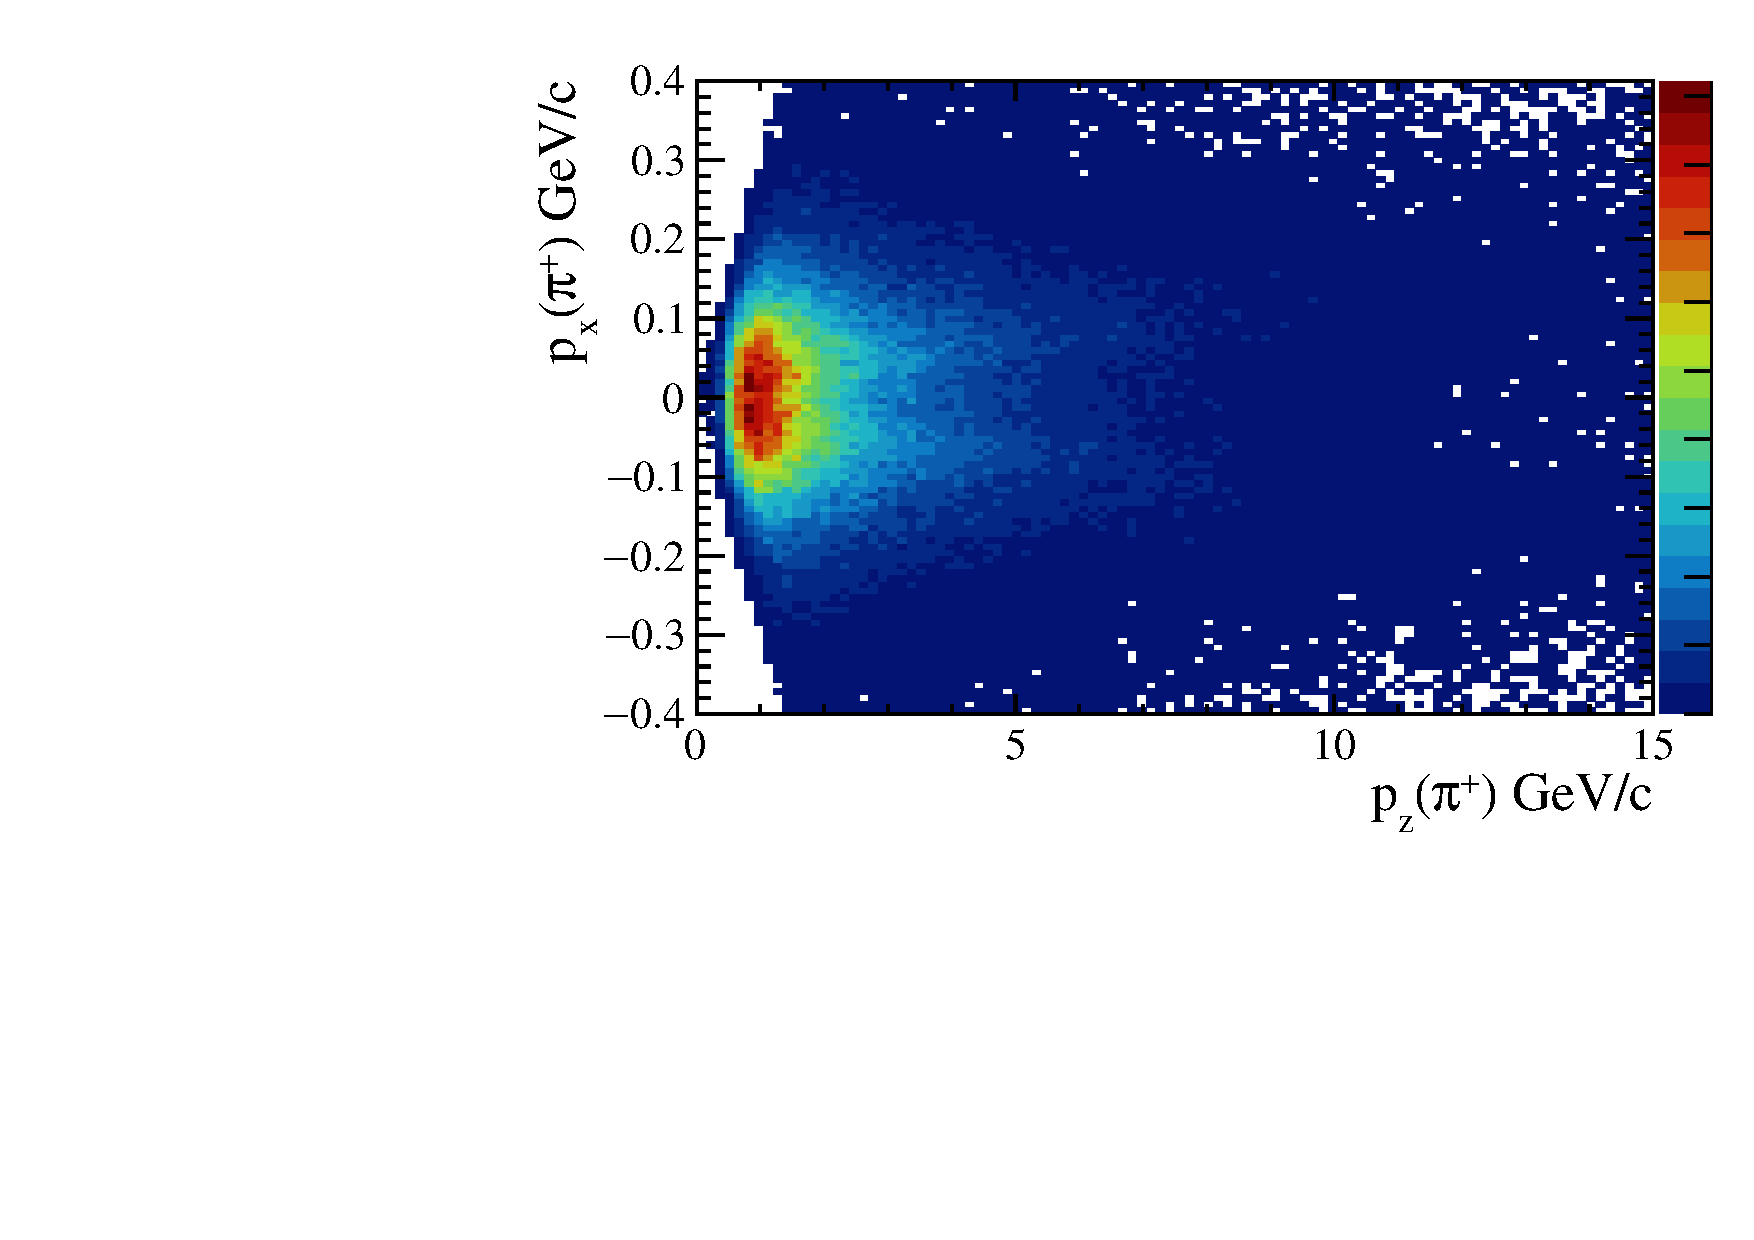
\includegraphics[width = 0.5\textwidth]{../work/RapidSimAnalysis/MomentumDependence/Plots/KK_Dst_PXPZ_Positive.pdf}}
                \subfloat{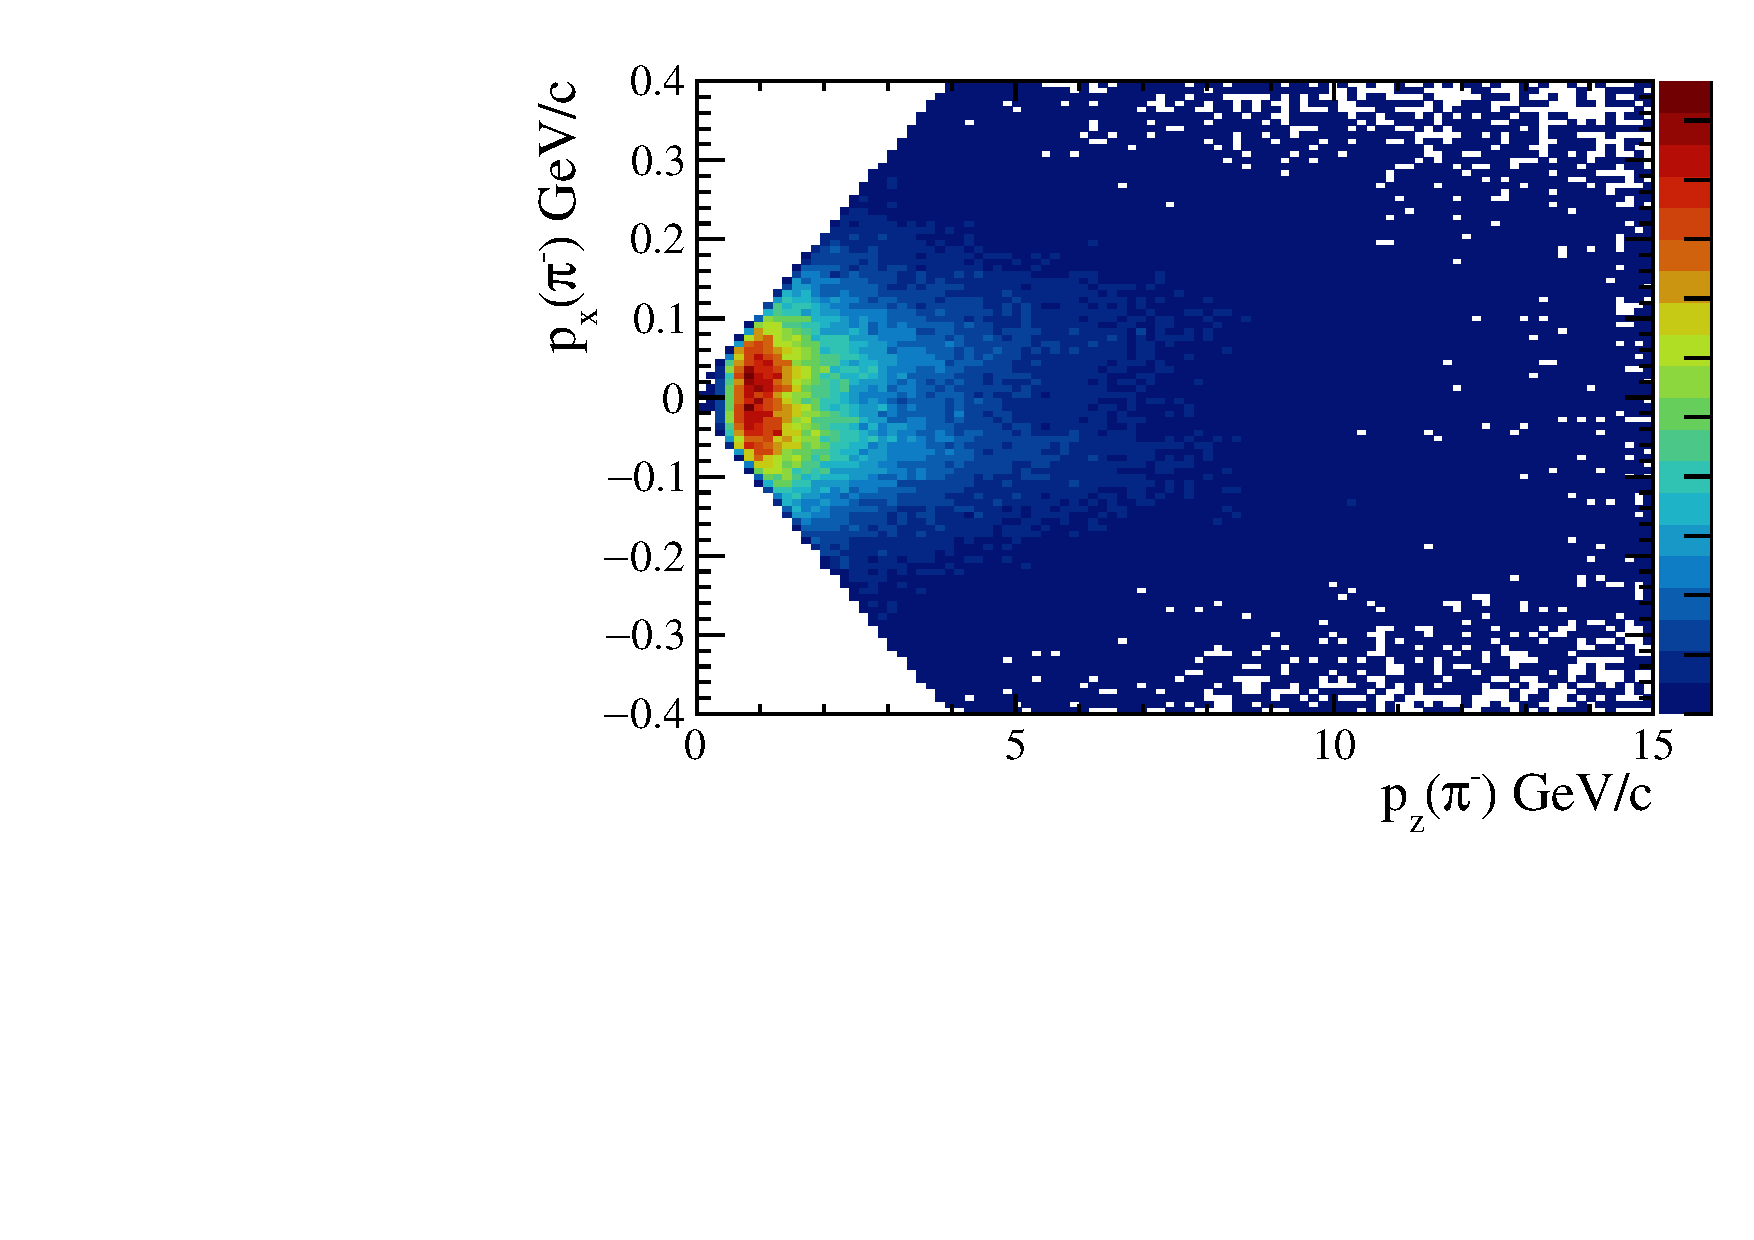
\includegraphics[width = 0.5\textwidth]{../work/RapidSimAnalysis/MomentumDependence/Plots/KK_Dst_PXPZ_Negative.pdf}}
                \caption{Positive and negative soft pion $p_x - p_z$ momentum plane for the $D^0\to K^-K^+$ sample.
                We remove negative soft pions from kinematic regions associated with $A_D(\vec{p}) = 1$.}
                \label{fig:detection}
        \end{figure}
        Subsequently, we calculate the weighting function using both techniques.

        We present  in Fig.~\ref{fig:weightsBeforeAfter} the distribution of the weighting function values using the two techniques we discussed.
        \begin{figure}[h!]
                \centering
                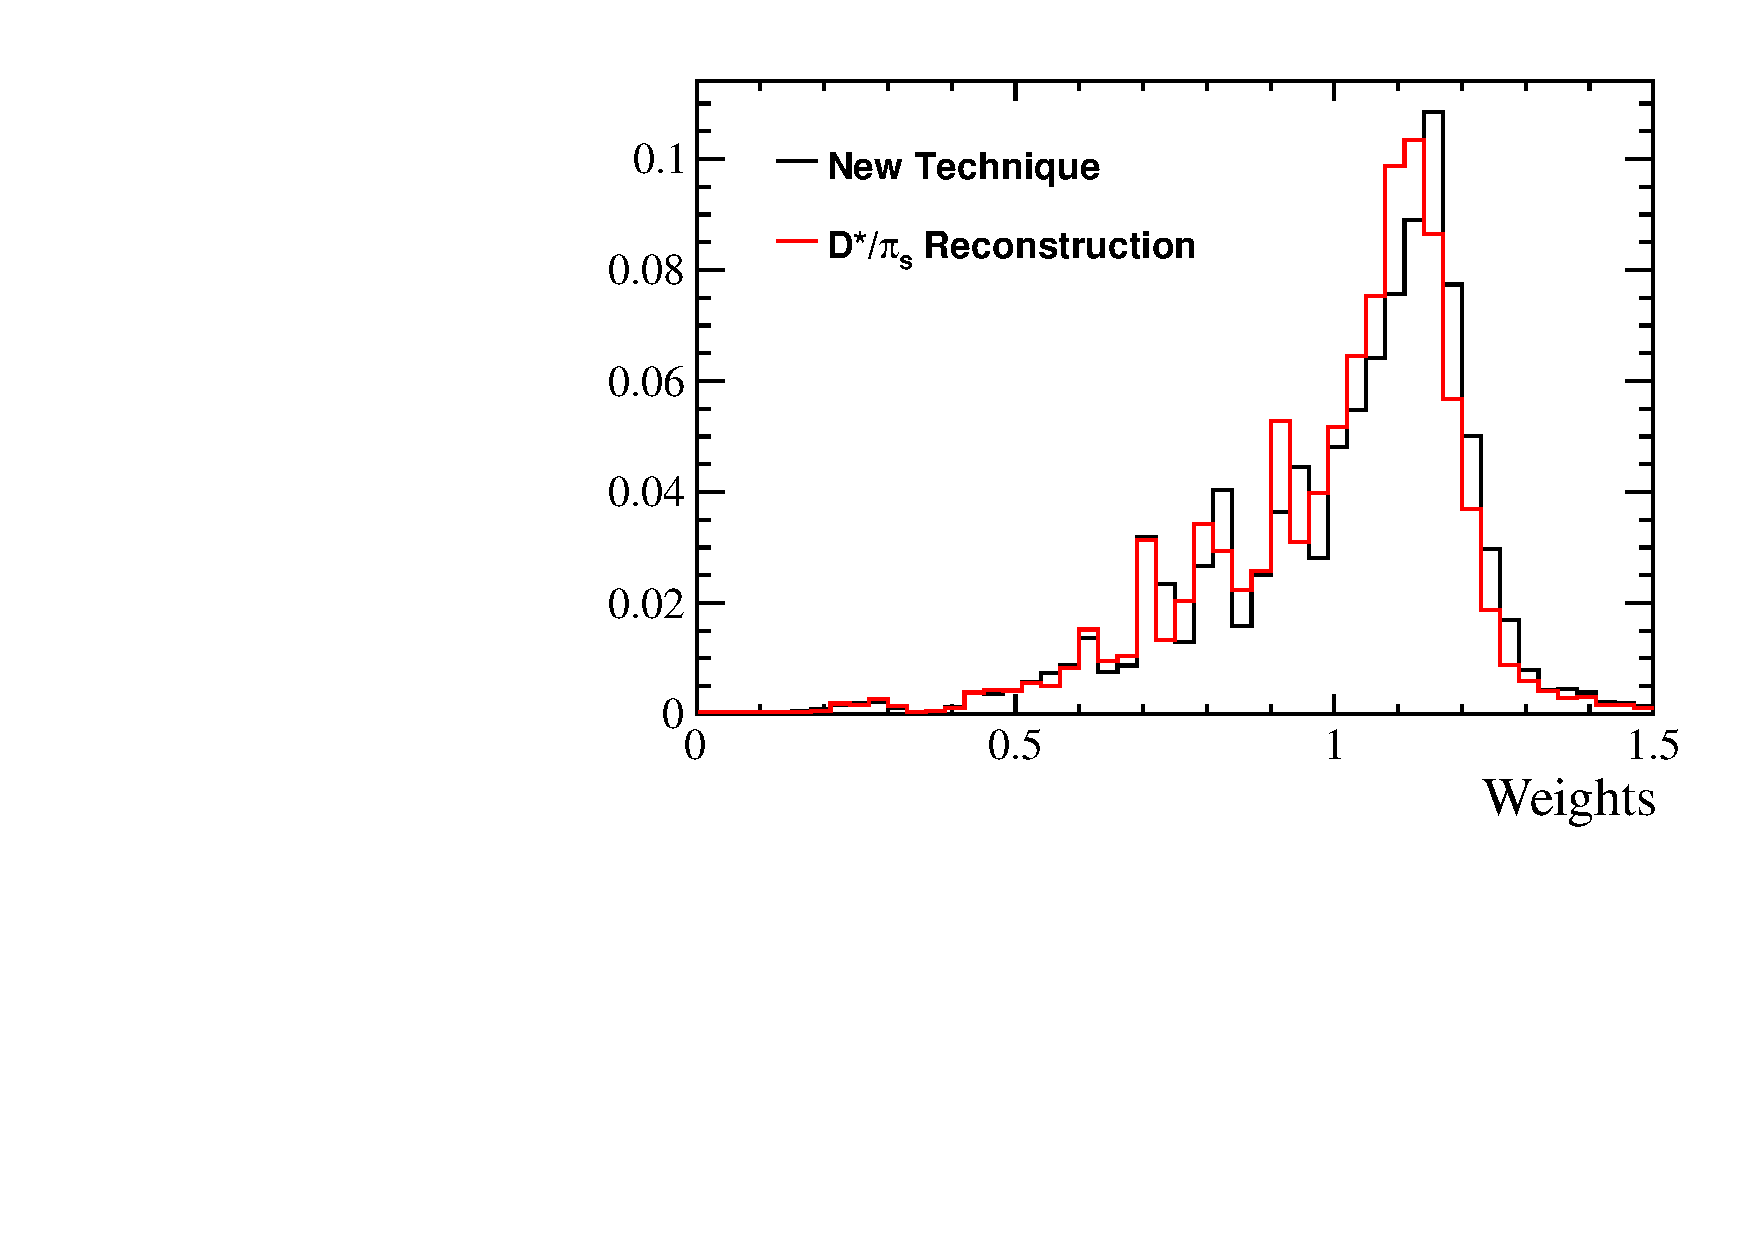
\includegraphics[width = 0.5\textwidth]{../work/RapidSimAnalysis/NewWeightingFunction/Plots/WeighsBeforeAfter.pdf}
                \caption{Distribution of weighting function values.
                The black histogram represents the new technique where we reconstruct $D^0$ candidates from either $K^-K^+$ or $\pi^-\pi^+$ while the red histogram represents the old weighting function where $D^0$ candidates were reconstructed using the $D^\star$ and the soft pion.}
                \label{fig:weightsBeforeAfter}
        \end{figure}
        As we can see the two weighting methods have subtle differences.
        Lastly, we present the $D^0$ kinematic distributions with and without weighting in Fig.~\ref{fig:D0Comparison}.
        \begin{figure}[h!]
                \centering
                \subfloat{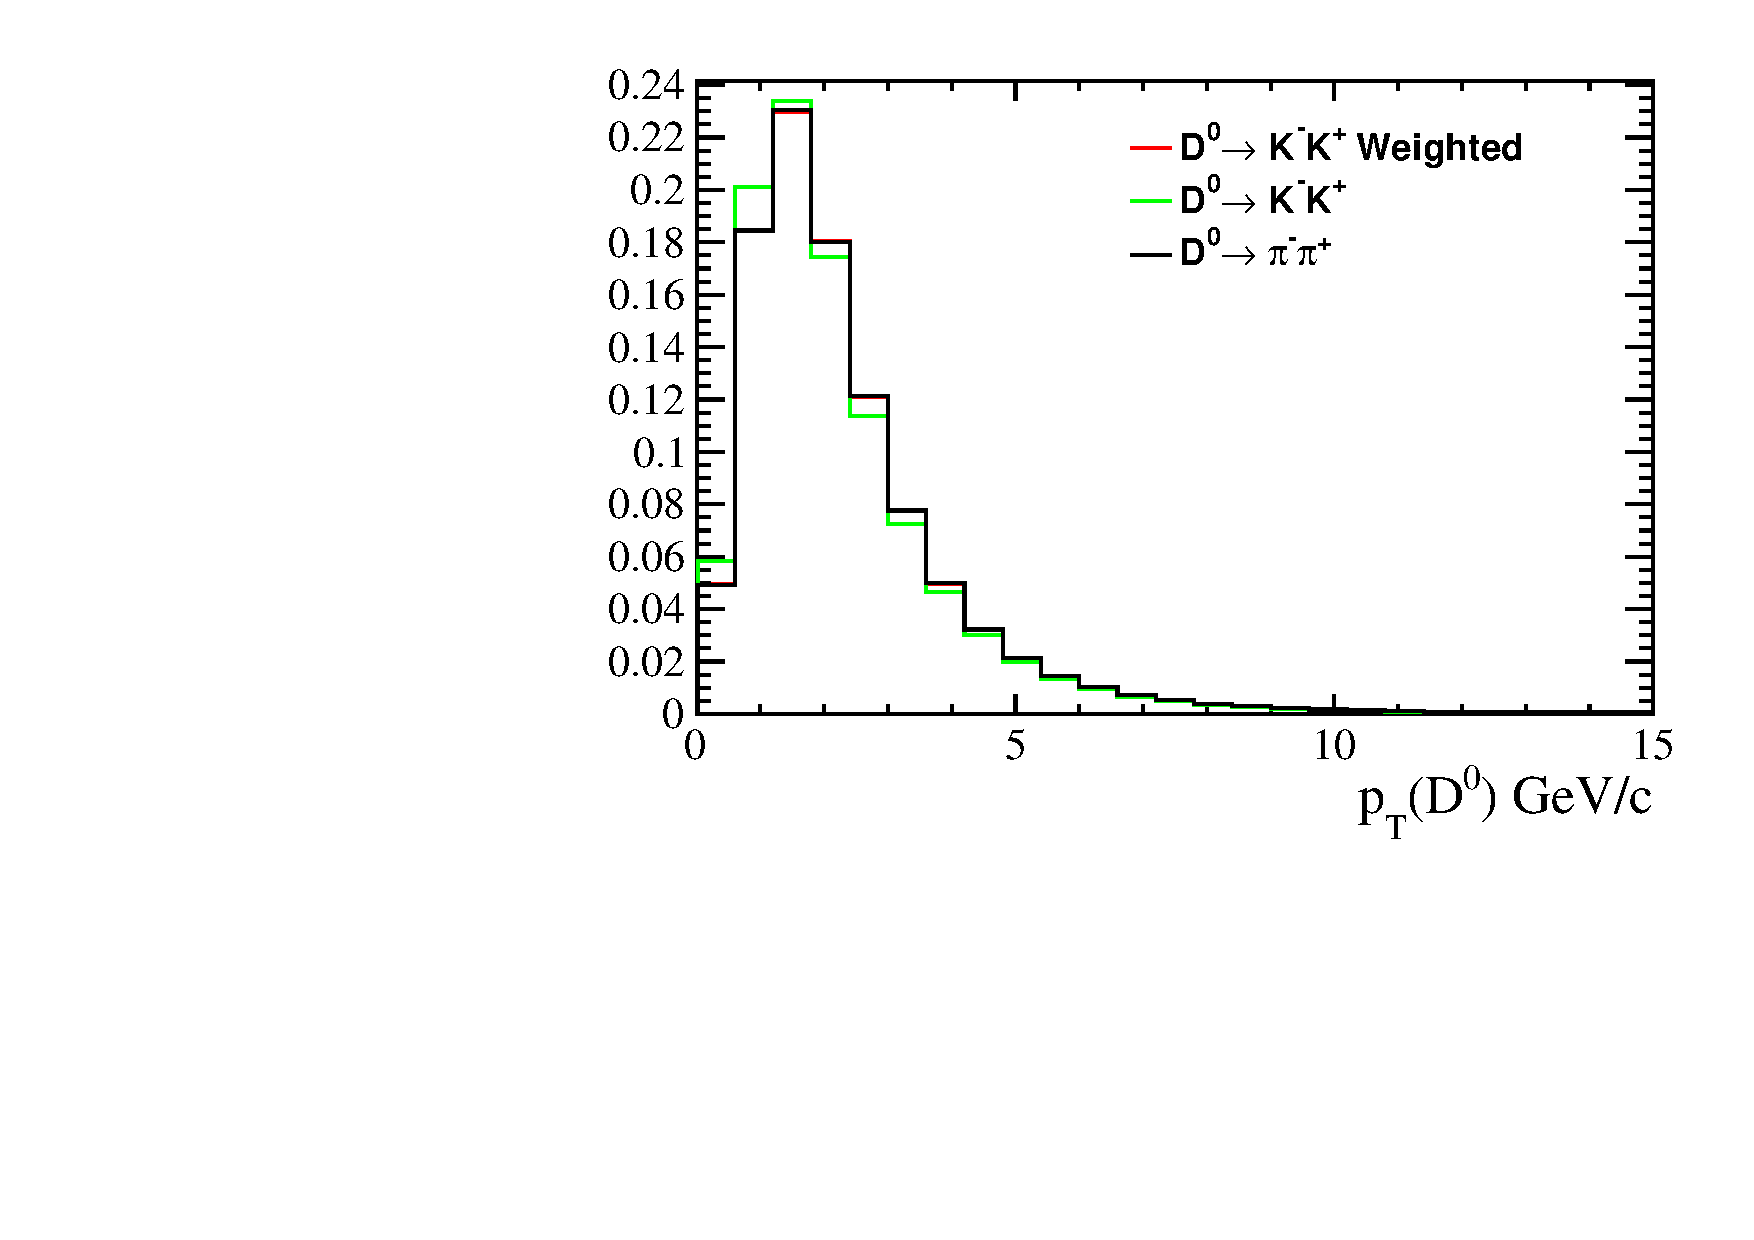
\includegraphics[width = 0.45\textwidth]{../work/RapidSimAnalysis/NewWeightingFunction/Plots/D0_PT_All.pdf}}
                \subfloat{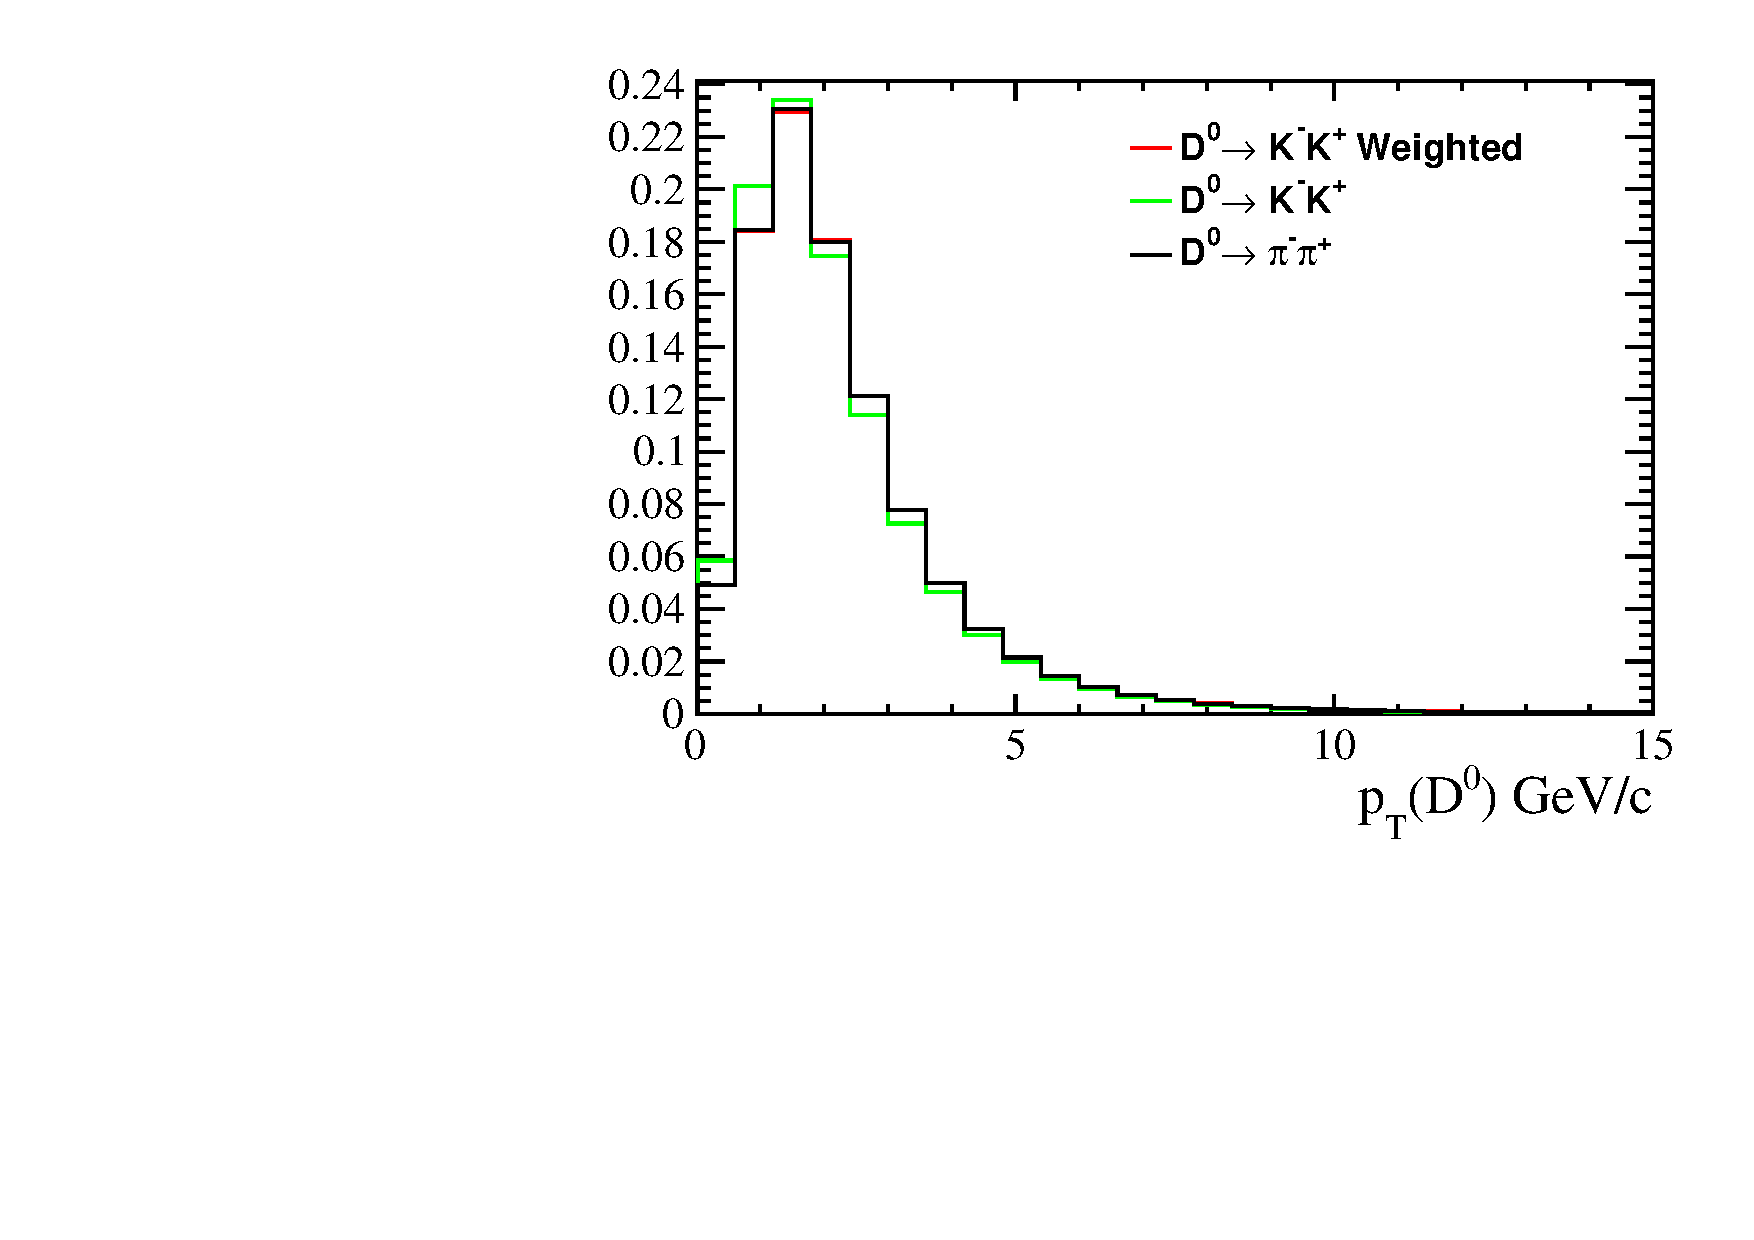
\includegraphics[width = 0.45\textwidth]{../work/RapidSimAnalysis/WeightingFunction/Plots/D0_PT_All.pdf}}
                \hfill
                \subfloat{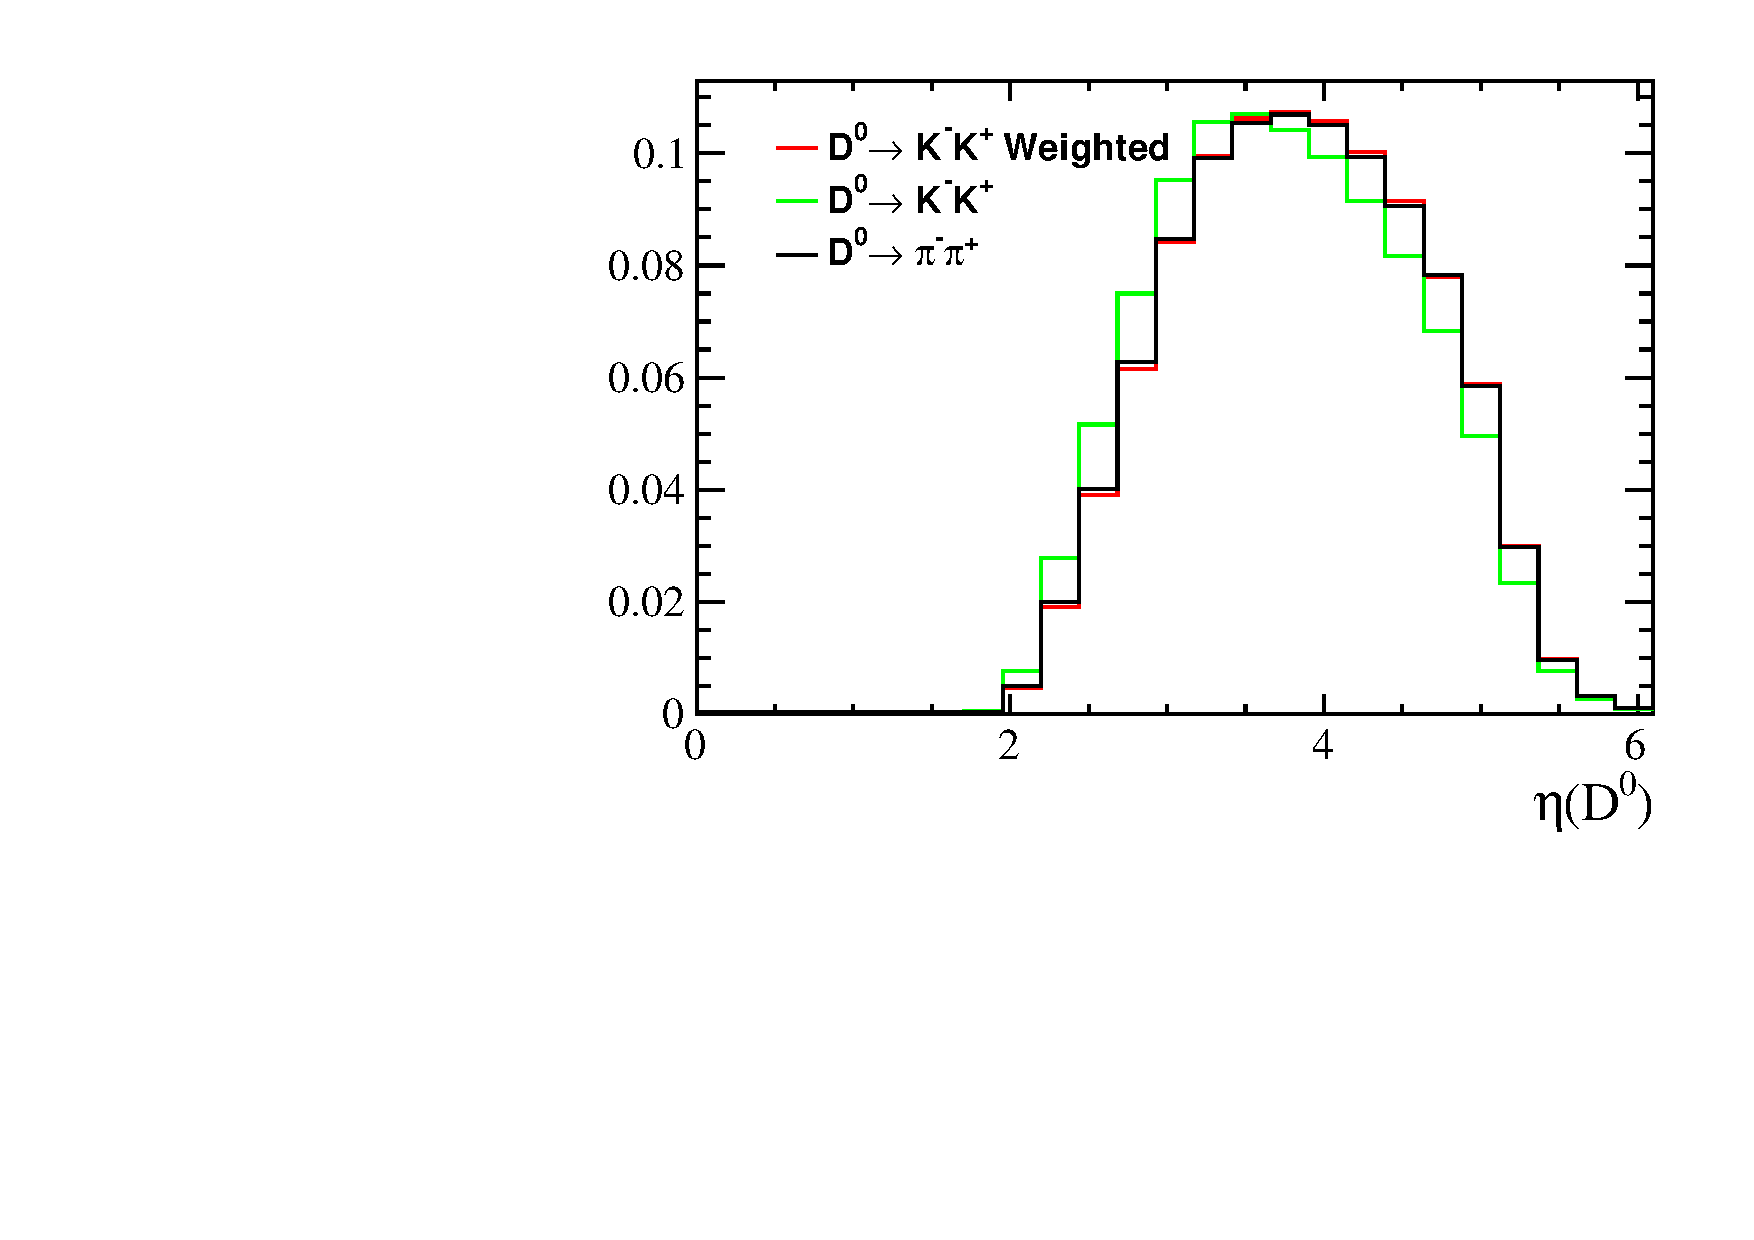
\includegraphics[width = 0.45\textwidth]{../work/RapidSimAnalysis/NewWeightingFunction/Plots/D0_eta_All.pdf}}
                \subfloat{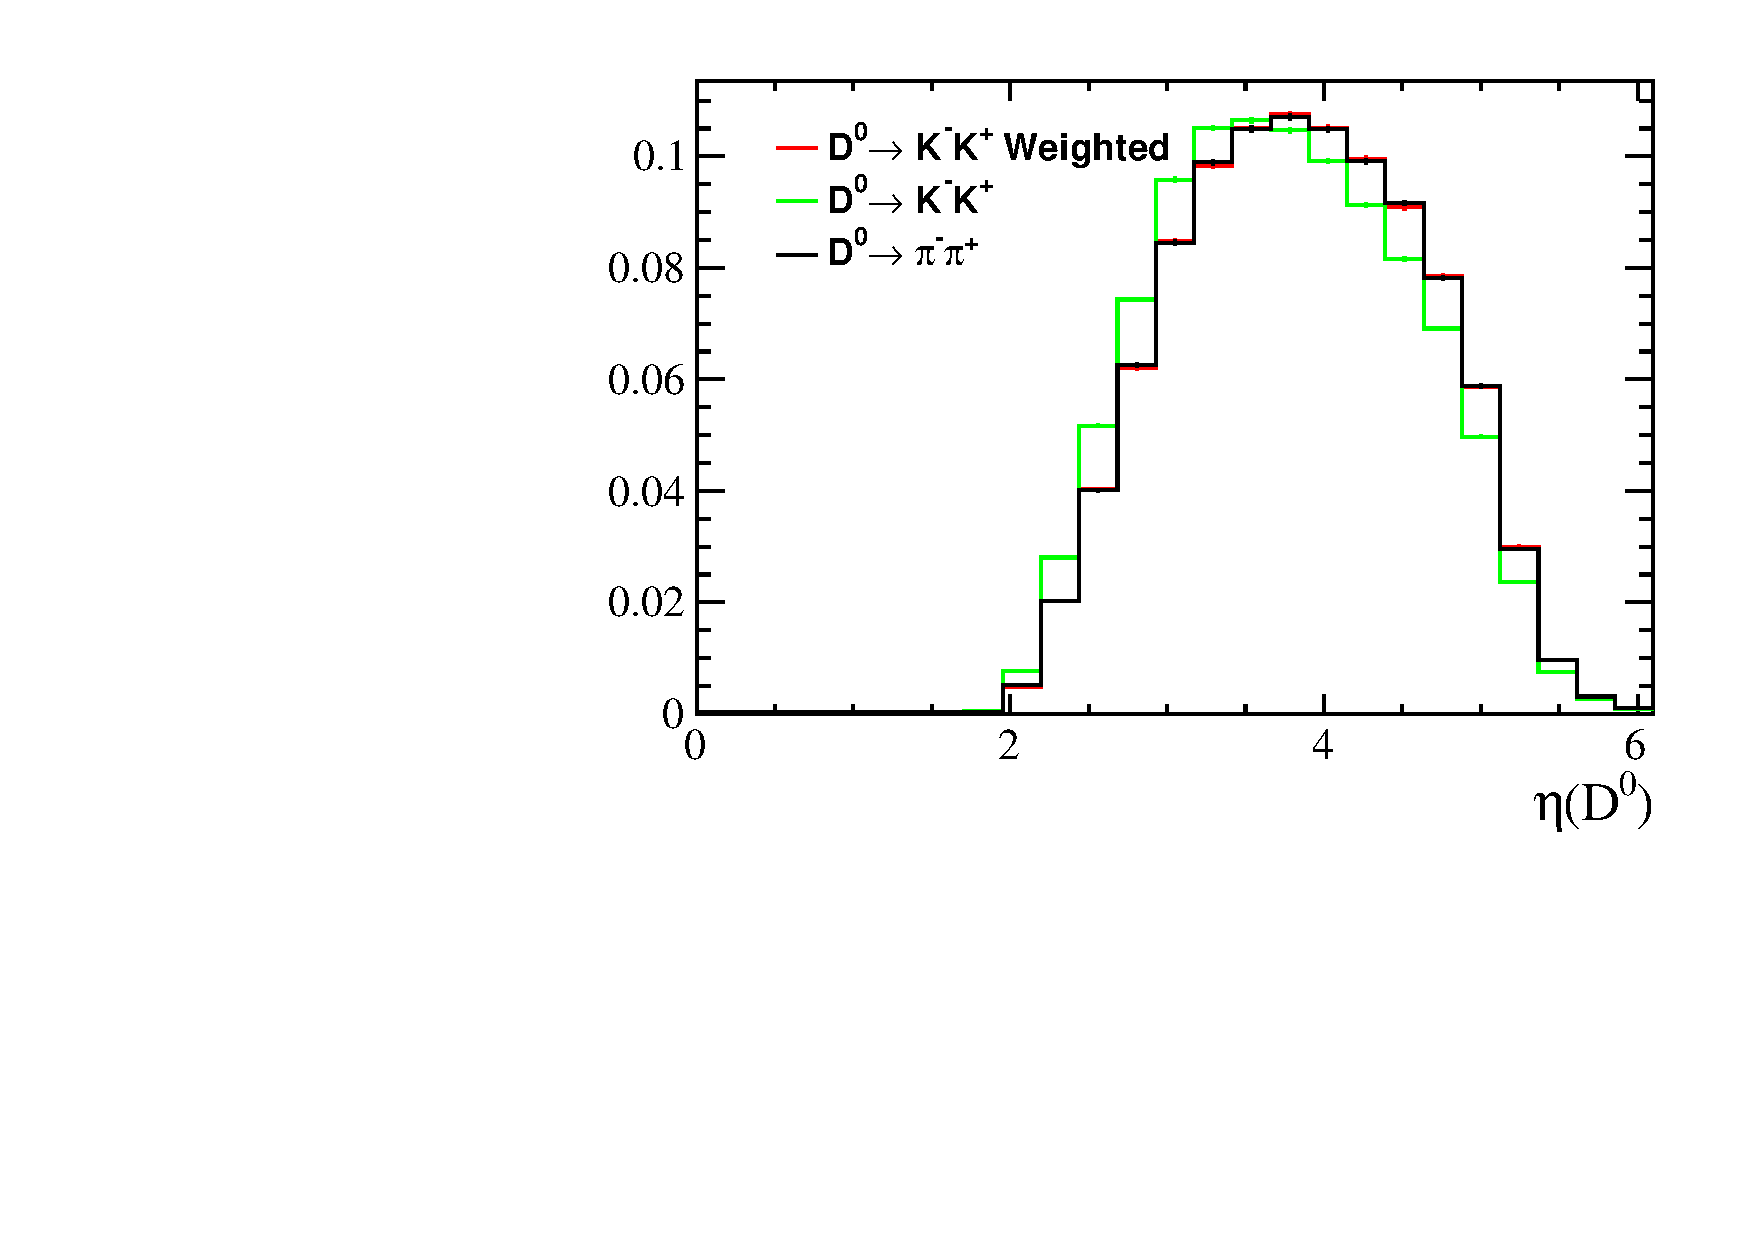
\includegraphics[width = 0.45\textwidth]{../work/RapidSimAnalysis/WeightingFunction/Plots/D0_eta_All.pdf}}
                \caption{Comparison of $D^0$ kinematics with and without weighting. On the left column we present we new weighting technique with $D^0$ candidates reconstructed from $K^-K^+$ and on the right the baseline technique.}
                \label{fig:D0Comparison}
        \end{figure}

        \pagebreak

        \subsection{Asymmetry calculation}
        Using the weighting function we can calculate the total asymmetry for $D^0\to K^-K^+$ and $D^0\to\pi^-\pi^+$ samples and compare to the unweighted result.
        The total asymmetry can be calculated through
        \begin{equation}
                A_\text{total} = \frac{N_+ - N_-}{N_+ + N_-}
        \end{equation}
        where for the case of unweighted samples, the number of positive and negative soft pion events are $N_+$ and $N_-$ respectively, and the uncertainties are given by $\sigma\left(N_\pm\right) = \sqrt{N_{\pm}}$.
        On the contrary, for weighted samples, we have
        \begin{equation}
                N_\pm = \sum_i w_i^\pm, \text{ and } \sigma\left(N_\pm\right) = \sqrt{\sum_i (w_i^\pm)^2}
        \end{equation} 
        and using propagation of uncertainties we can calculate the total asymmetry error
        \begin{equation}
                \sigma\left(A_{\text{total}} ^2\right) = \left(\pdv{A_{\text{total}}}{N^+}\sigma\left(N^+\right)\right)^2 + \left(\pdv{A_{\text{total}}}{N^-}\sigma\left(N^-\right)\right)^2
        \end{equation}

        We present the calculated asymmetries for the $D^0\to K^-K^+$ sample in Tab.~\ref{tab:asymmetries_total}
        \begin{center}
                \begin{tabular}{c|c|c}
                        Technique & Weighted & Unweighted\\
                        \hline\hline
                        Not associated & $A_\text{total} = 0.14726 \pm 0.00050$ & \multirow{2}{*}{$A_\text{total} = 0.16268 \pm 0.00049$}\\
                        \cline{1-2}
                        Associated with $\pi_s$ & $A_\text{total} = 0.14994 \pm 0.00050$ & \\
                \end{tabular}
                \captionof{table}{$A_\text{total}$ for the $D^0\to K^-K^+$ sample with and without weighting.}
                \label{tab:asymmetries_total}
        \end{center}
        and for the $D^0\to \pi^-\pi^+$ sample we get
        \begin{equation}
                A_\text{total} = 0.24571 \pm 0.00053
        \end{equation} 

        If the effect of the detection asymmetry is properly canceled, then he estimated total asymmetry difference should be $\Delta A_\text{total} = \Delta A_{CP} = -0.1$, according to the $CP$ asymmetries we introduced. 
        We present the results of the total asymmetry difference in Tab.~\ref{tab:asymmetry_difference} as well as the deviation from the expected value.
        Both weighting techniques appear to correct the measurement of $\Delta A_\text{total}$, however, there is much improvement between the previous weighting function and the new one.
        \begin{center}
                \begin{tabular}{c|c|c|c}
                        Technique& & Weighted & Unweighted\\
                        \hline\hline
                        \multirow{2}{*}{Not associated} & $\Delta A_\text{total}$ & $-0.09845 \pm 0.00073$ & \\
                        & Deviation $(\sigma)$ & $2.12$ & $-0.08303 \pm 0.00072$\\
                        \cline{1-3}
                        \multirow{2}{*}{Associated with $\pi_s$} & $\Delta A_\text{total}$ & $-0.09578 \pm 0.00073$ & $23.6$\\
                        & Deviation $(\sigma)$ & $5.78$ & \\
                \end{tabular}
                \captionof{table}{Total asymmetry difference with and without weights.
                We present both weighting procedures, before and after the detection asymmetry.}
                \label{tab:asymmetry_difference}
        \end{center}


        \subsection{Particle Gun analysis}
        The final test of the weighting function in Eq.~\ref{eq:weighting} is the implementation on samples generated with Particle Gun.
        In these samples there is no $CP$ asymmetry, however the simulation includes a detection asymmetry for soft pions as shown in Fig.~\ref{fig:detection_pgun}.
        \begin{figure}[h!]
                \centering
                \subfloat{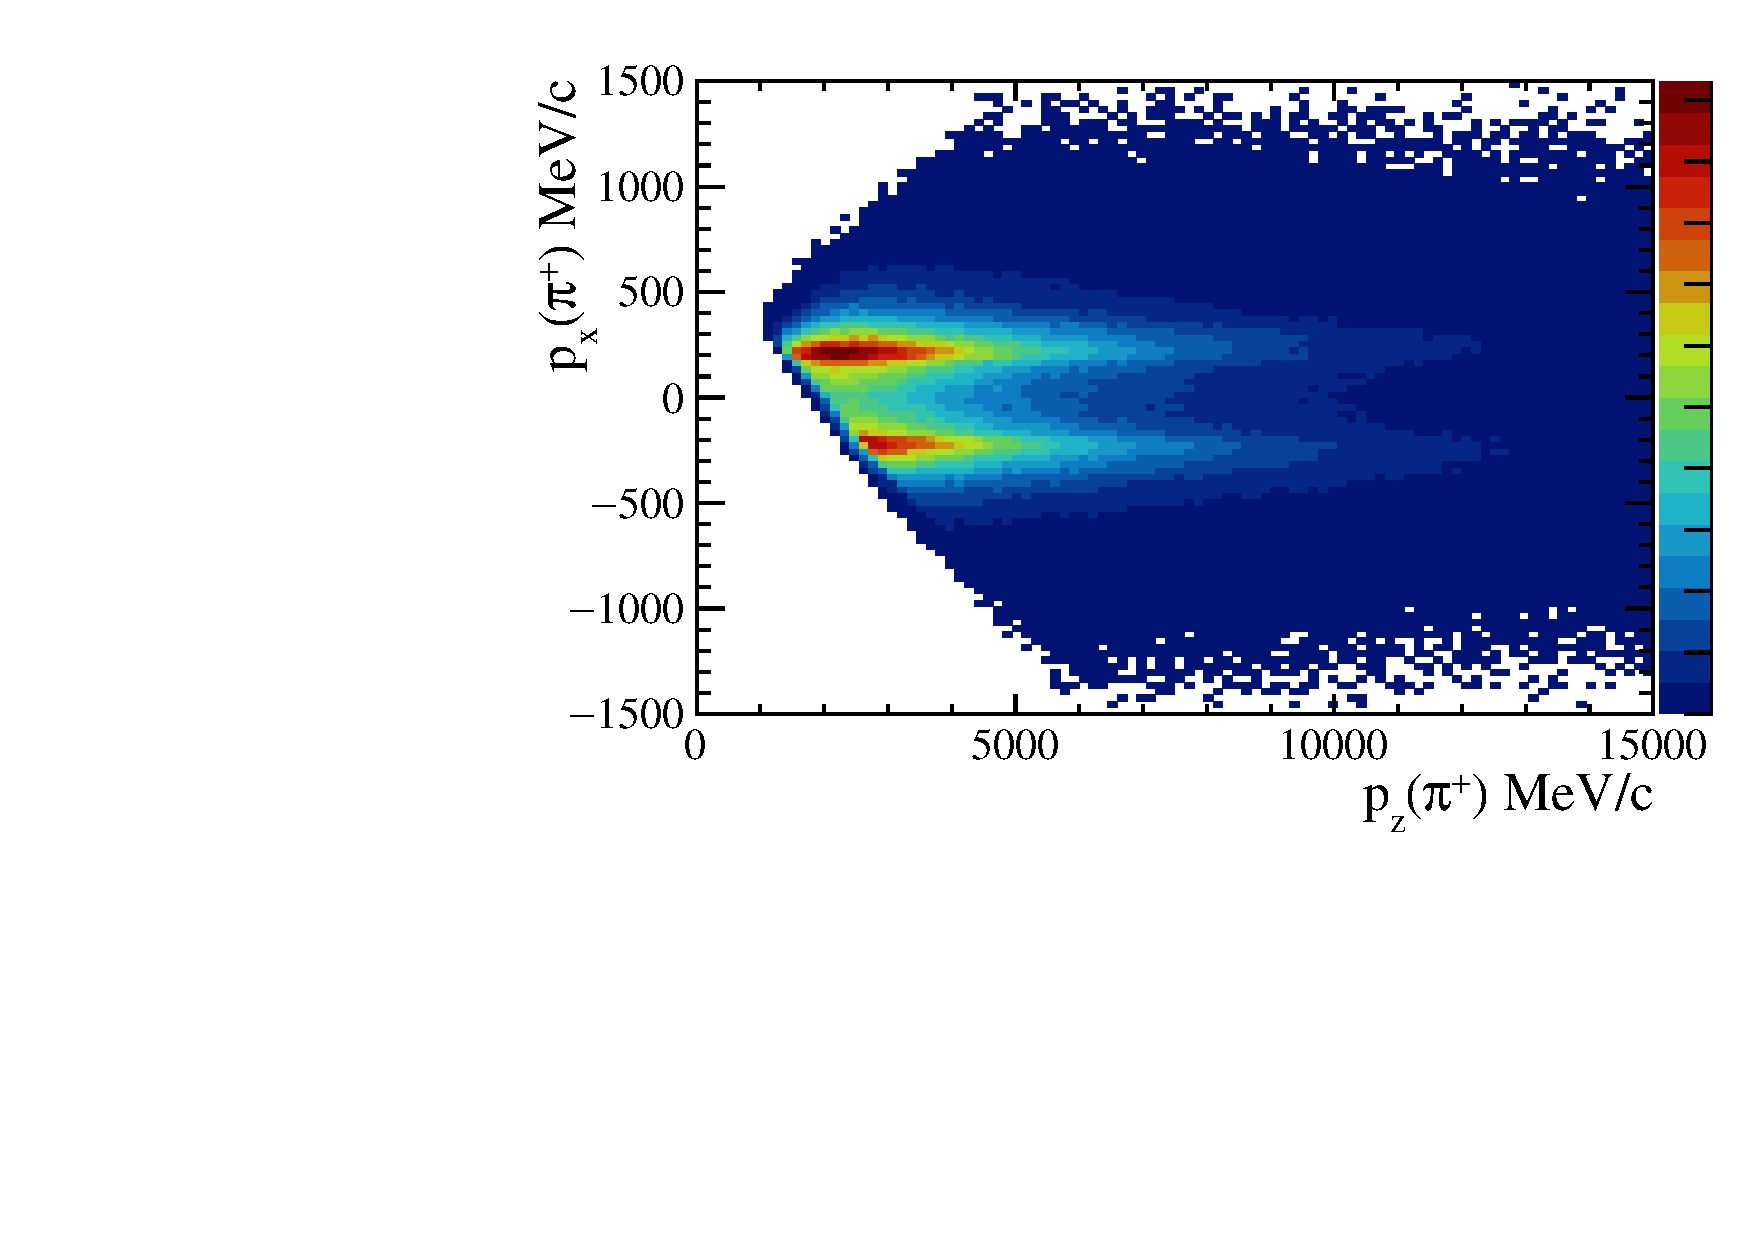
\includegraphics[width = 0.5\textwidth]{../work/RapidSimAnalysis/PGunAnalysis/Plots/KK_Dst_PXPZ_Positive.pdf}}
                \subfloat{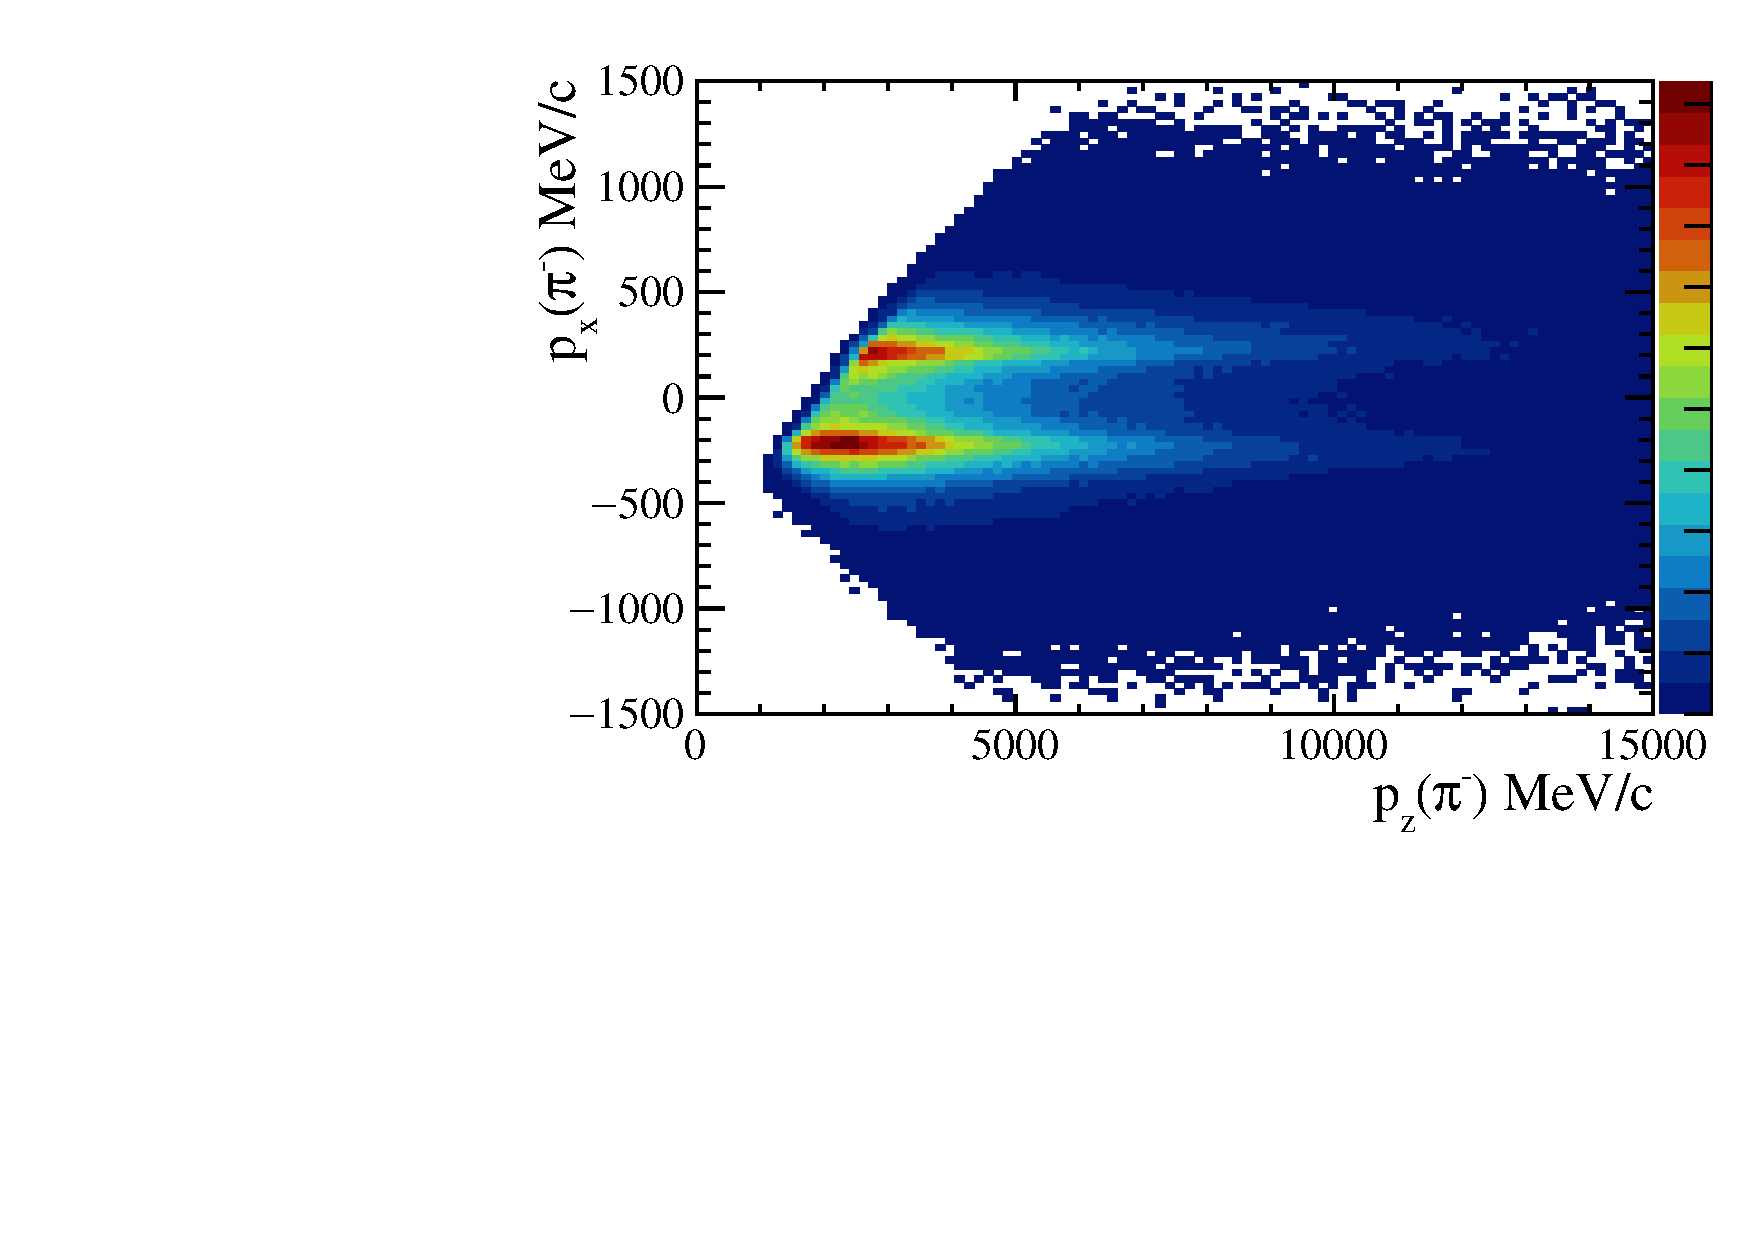
\includegraphics[width = 0.5\textwidth]{../work/RapidSimAnalysis/PGunAnalysis/Plots/KK_Dst_PXPZ_Negative.pdf}}
                \caption{We present the positive (left) and negative (right) soft pion $p_x - p_z$ momentum planes for the 2018 $D^0\to K^-K^+$ with up magnet polarity sample generated using Particle Gun.}
                \label{fig:detection_pgun}
        \end{figure}

        We test the new weighting technique on Particle Gun data with different magnet polarities.
        We present in Tab.~\ref{tab:2015}, \ref{tab:2016}, \ref{tab:2017} and \ref{tab:2018} the $A_\text{total}$ for various $D^0\to K^-K^+$ samples, and for $D^0\to \pi^-\pi^+$ in Tab.~\ref{tab:20152018}.
        \begin{center}
                \begin{tabular}{c|c|c}
                        Year & Polarity & $A_\text{total}$\\
                        \hline\hline
                        \multirow{2}{*}{2015} & Down & $0.00284 \pm 0.00048$\\
                        \cline{2-3}
                        & Up & $-0.00033\pm 0.00048$\\
                        \hline
                        \multirow{2}{*}{2016} & Down & $0.00296\pm 0.00049$\\
                        \cline{2-3}
                        & Up & $-0.00130\pm 0.00048$\\
                        \hline
                        \multirow{2}{*}{2017} & Down & $0.00349\pm 0.00053$\\
                        \cline{2-3}
                        & Up & $-0.00091\pm 0.00052$\\
                        \hline
                        \multirow{2}{*}{2018} & Down & $0.00260\pm 0.00053$\\
                        \cline{2-3}
                        & Up & $-0.00024\pm 0.00052$\\
                \end{tabular}
                \captionof{table}{Total asymmetry of 2015-2018 $D^0\to\pi^-\pi^+$ samples with both magnet polarities.}
                \label{tab:20152018}
        \end{center}
        \begin{center}
                \begin{tabular}{c|c|c|c}
                        Polarity & Technique & Weighted & Unweighted\\
                        \hline\hline
                        \multirow{2}{*}{Down} & Not associated & $A_\text{total} = 0.00300 \pm 0.00053$ & \multirow{2}{*}{$A_\text{total} = 0.00272 \pm 0.00053$}\\
                        \cline{2-3}
                        & Associated with $\pi_s$ & $A_\text{total} = 0.00306 \pm 0.00053$ & \\
                        % \cline{1-3}
                        \hline
                        \multirow{2}{*}{Up} & Not associated & $A_\text{total} = - 0.00063 \pm 0.00053$ & \multirow{2}{*}{$A_\text{total} = - 0.00018 \pm 0.00052$}\\
                        \cline{2-3}
                        & Associated with $\pi_s$ & $A_\text{total} = - 0.00031 \pm 0.00053$ & \\
                \end{tabular}
                \captionof{table}{We present the $A_\text{total}$ for the $D^0\to K^-K^+$ Particle Gun 2015 sample weighted using the two techniques and unweighted for both polarities.}
                \label{tab:2015}
        \end{center}
        \begin{center}
                \begin{tabular}{c|c|c|c}
                        Polarity & Technique & Weighted & Unweighted\\
                        \hline\hline
                        \multirow{2}{*}{Down} & Not associated & $A_\text{total} = 0.00359 \pm 0.00052$ & \multirow{2}{*}{$A_\text{total} = 0.00331 \pm 0.00052$}\\
                        \cline{2-3}
                        & Associated with $\pi_s$ & $A_\text{total} = 0.00339 \pm 0.00052$ & \\
                        % \cline{1-3}
                        \hline
                        \multirow{2}{*}{Up} & Not associated & $A_\text{total} = - 0.00122 \pm 0.00053$ & \multirow{2}{*}{$A_\text{total} = - 0.00082 \pm 0.00053$}\\
                        \cline{2-3}
                        & Associated with $\pi_s$ & $A_\text{total} = - 0.00105 \pm 0.00053$ & \\
                \end{tabular}
                \captionof{table}{We present the $A_\text{total}$ for the $D^0\to K^-K^+$ Particle Gun 2016 sample weighted using the two techniques and unweighted for both polarities.}
                \label{tab:2016}
        \end{center}
        \begin{center}
                \begin{tabular}{c|c|c|c}
                        Polarity & Technique & Weighted & Unweighted\\
                        \hline\hline
                        \multirow{2}{*}{Down} & Not associated & $A_\text{total} = 0.00208\pm 0.00056$ & \multirow{2}{*}{$A_\text{total} = 0.00191\pm 0.00056$}\\
                        \cline{2-3}
                        & Associated with $\pi_s$ & $A_\text{total} = 0.00186\pm 0.00056$ & \\
                        % \cline{1-3}
                        \hline
                        \multirow{2}{*}{Up} & Not associated & $A_\text{total} = - 0.00095\pm 0.00056$ & \multirow{2}{*}{$A_\text{total} = - 0.00059 \pm 0.00056$}\\
                        \cline{2-3}
                        & Associated with $\pi_s$ & $A_\text{total} = - 0.00109\pm 0.00056$ & \\
                \end{tabular}
                \captionof{table}{We present the $A_\text{total}$ for the $D^0\to K^-K^+$ Particle Gun 2017 sample weighted using the two techniques and unweighted for both polarities.}
                \label{tab:2017}
        \end{center}
        \begin{center}
                \begin{tabular}{c|c|c|c}
                        Polarity & Technique & Weighted & Unweighted\\
                        \hline\hline
                        \multirow{2}{*}{Down} & Not associated & $A_\text{total} = 0.00265 \pm 0.00056$ & \multirow{2}{*}{$A_\text{total} = 0.00246 \pm 0.00056$}\\
                        \cline{2-3}
                        & Associated with $\pi_s$ & $A_\text{total} = 0.00281\pm 0.00056$ & \\
                        % \cline{1-3}
                        \hline
                        \multirow{2}{*}{Up} & Not associated & $A_\text{total} = - 0.00023\pm 0.00056$ & \multirow{2}{*}{$A_\text{total} = 0.00002\pm 0.00056$}\\
                        \cline{2-3}
                        & Associated with $\pi_s$ & $A_\text{total} = - 0.00002\pm 0.00056$ & \\
                \end{tabular}
                \captionof{table}{We present the $A_\text{total}$ for the $D^0\to K^-K^+$ Particle Gun 2018 sample weighted using the two techniques and unweighted for both polarities.}
                \label{tab:2018}
        \end{center}

        We calculate $\Delta A_{CP}$ for all samples and subsequently perform a weighted average to obtain our final results.
        We present the average of all samples in Tab.~\ref{tab:average}.
        As we can see, the weighting function where $D^0$ is associated with $\pi_s$ introduced bias to our final results.
        Moreover, we observe that in this instance, the new weighting technique does not improve the $\Delta A_\text{total}$ average value.

        \begin{center}
                \begin{tabular}{c|c|c|c|c|c}
                        Year & Polarity & Technique & & Weighted & Unweighted\\
                        \hline\hline
                        \multirow{8}{*}{2015} & \multirow{4}{*}{Down} & \multirow{2}{*}{Not associated} & $\Delta A_\text{total}$ & $0.00016\pm 0.00072$& \\
                        & & & Deviation $(\sigma)$ & 0.22& $-0.00012\pm 0.00072$\\
                        \cline{3-5}
                        & & \multirow{2}{*}{Associated with $\pi_s$} & $\Delta A_\text{total}$ & $0.00022\pm 0.00072$& -0.17\\
                        & & & Deviation $(\sigma)$ & 0.31& \\
                        \cline{2-6}
                        & \multirow{4}{*}{Up} & \multirow{2}{*}{Not associated} & $\Delta A_\text{total}$ & $-0.00030\pm 0.00072$& \\
                        & & & Deviation $(\sigma)$ & -0.30& $0.00015\pm 0.00072$\\
                        \cline{3-5}
                        & & \multirow{2}{*}{Associated with $\pi_s$} & $\Delta A_\text{total}$ & $0.00002\pm 0.00072$& 0.15\\
                        & & & Deviation $(\sigma)$ & 0.02& \\
                        \hline

                        \multirow{8}{*}{2016} & \multirow{4}{*}{Down} & \multirow{2}{*}{Not associated} & $\Delta A_\text{total}$ & $0.00063\pm 0.00071$& \\
                        & & & Deviation $(\sigma)$ & 0.89& $0.00035\pm 0.00071$ \\
                        \cline{3-5}
                        & & \multirow{2}{*}{Associated with $\pi_s$} & $\Delta A_\text{total}$ & $0.00043\pm 0.00071$& 0.49\\
                        & & & Deviation $(\sigma)$ & 0.61& \\
                        \cline{2-6}
                        & \multirow{4}{*}{Up} & \multirow{2}{*}{Not associated} & $\Delta A_\text{total}$ & $0.00008\pm 0.00072$& \\
                        & & & Deviation $(\sigma)$ & 0.11& $0.00048\pm 0.00072$\\
                        \cline{3-5}
                        & & \multirow{2}{*}{Associated with $\pi_s$} & $\Delta A_\text{total}$ & $0.00025\pm 0.00072$& 0.67\\
                        & & & Deviation $(\sigma)$ & 0.35& \\
                        \hline

                        \multirow{8}{*}{2017} & \multirow{4}{*}{Down} & \multirow{2}{*}{Not associated} & $\Delta A_\text{total}$ & $-0.00141\pm 0.00077$& \\
                        & & & Deviation $(\sigma)$ & 1.83& $-0.00158\pm 0.00077$\\
                        \cline{3-5}
                        & & \multirow{2}{*}{Associated with $\pi_s$} & $\Delta A_\text{total}$ & $-0.00163\pm 0.00077$& -2.05\\
                        & & & Deviation $(\sigma)$ & -2.12& \\
                        \cline{2-6}
                        & \multirow{4}{*}{Up} & \multirow{2}{*}{Not associated} & $\Delta A_\text{total}$ & $-0.00004\pm 0.00076$& \\
                        & & & Deviation $(\sigma)$ & 0.05& $0.00032\pm 0.00076$\\
                        \cline{3-5}
                        & & \multirow{2}{*}{Associated with $\pi_s$} & $\Delta A_\text{total}$ & $-0.00018\pm 0.00076$& 0.42\\
                        & & & Deviation $(\sigma)$ & 0.24& \\
                        \hline

                        \multirow{8}{*}{2018} & \multirow{4}{*}{Down} & \multirow{2}{*}{Not associated} & $\Delta A_\text{total}$ & $0.00004\pm 0.00077$& \\
                        & & & Deviation $(\sigma)$ & 0.05& $-0.00014\pm 0.00077$\\
                        \cline{3-5}
                        & & \multirow{2}{*}{Associated with $\pi_s$} & $\Delta A_\text{total}$ & $0.00021\pm 0.00077$& 0.18\\
                        & & & Deviation $(\sigma)$ & 0.27& \\
                        \cline{2-6}
                        & \multirow{4}{*}{Up} & \multirow{2}{*}{Not associated} & $\Delta A_\text{total}$ & $0.00001\pm 0.00076$& \\
                        & & & Deviation $(\sigma)$ & 0.01& $0.00026\pm 0.00076$\\
                        \cline{3-5}
                        & & \multirow{2}{*}{Associated with $\pi_s$} & $\Delta A_\text{total}$ & $0.00022\pm 0.00076$& 0.34\\
                        & & & Deviation $(\sigma)$ & 0.29& \\
                        \hline
                \end{tabular}
                \captionof{table}{We present the values of $\Delta A_\text{total}$ for all samples.}
                \label{tab:all}
        \end{center}

        \begin{table}[htbp]
                \begin{adjustbox}{center}
                        \begin{tabular}{c|c|c|c|c|c}
                                Year & Polarity & Technique & & Weighted & Unweighted\\
                                \hline\hline
                                \multirow{4}{*}{Average} & \multirow{4}{*}{Both} & \multirow{2}{*}{Not associated} & $\Delta A_\text{total}$ & $-0.000084\pm 0.000262$& \\
                                & & & Deviation $(\sigma)$ & 0.32& $-0.000015\pm 0.000262$\\
                                \cline{3-5}
                                & & \multirow{2}{*}{Associated with $\pi_s$} & $\Delta A_\text{total}$ & $-0.000036\pm 0.000262$& 0.057\\
                                & & & Deviation $(\sigma)$ & 0.14& \\
                        \end{tabular}
                \end{adjustbox}
                \captionof{table}{We present the weighted average value of $\Delta A_{CP}$ for all samples.}
                \label{tab:average}
        \end{table}

        \section{Conclusions}
        As demonstrated the weighting function allows us to keep events with kinematics associated with large detection asymmetries without affecting our results.

        From the analysis of the RapidSim data we observe a reduction in the deviation of $\Delta A_\text{total}$ when applying the old weighting function (association with $\pi_s$), however, by employing the new weighting technique the deviation reduces by more than a factor of 10.
        Thus, from this data sample we conclude that the new weighting technique (not associated with $\pi_s$) is much more effective.

        Furthermore, we employed the weighting functions to Particle Gun data in order to study a more realistic scenario.
        For these specific datasets we noticed that both weighting functions do not improve the $\Delta A_\text{total}$ result after averaging all samples and all magnet polarities.
        

        In conclusion, the weighting function we examined needs to be studied further before being employed on real Run-3 data. 
        For the RapidSim case we noticed an improvement of the $\Delta A_\text{total}$ result, but not for the Particle Gun case with the current statistics.
        We noticed that the effect of $A_D$ is canceled after averaging both magnet polarities, thus, further investigations are needed.
        
        \pagebreak
        \nocite{*}
        \printbibliography[notcategory=cited]
        \addcontentsline{toc}{chapter}{Bibliography}
\end{document}